% No New page; first instance
\visHeader
\subsection[An Abstract Definition (Visual)]{An Abstract Definition; Modeling with \mbox{Enterprise Architect}}
\label{sec:staticAbstract}

% Rewrite assuming user has not worked through chapter one!
\begin{enumerate}
\item[$\blacktriangleright$] \hypertarget{static vis}{Switch} Make sure Eclipse is open in the same workspace as Part I. If you're just starting, start a New metamodel project. From either, open Enterprise Architect (EA) with the \texttt{Demo.eap} file. In EA, select \texttt{Demo} and click on the button \texttt{Add a Package} as depicted in Fig.~\ref{fig:new_package}.

\begin{figure}[htbp]
	\centering
  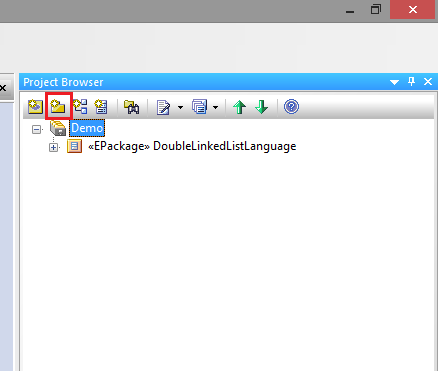
\includegraphics[width=0.7\textwidth]{EA_addPackage}
	\caption{Add a new package to \texttt{Demo}.}
	\label{fig:new_package}
\end{figure}

\item[$\blacktriangleright$] In the dialogue that pops up (Fig.~\ref{fig:new_package_name}), choose \texttt{Class View}, enter \texttt{Learning\-Box\-Language} as the name of the new package and click \texttt{OK}.

\begin{figure}[htbp]
	\centering
    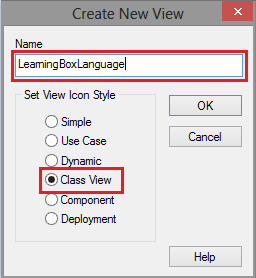
\includegraphics[width=0.3\textwidth]{EA_namePackage.png}
	\caption{Enter the name of the new package.}
	\label{fig:new_package_name}
\end{figure}
\end{enumerate}
\FloatBarrier

In your EA workspace the \texttt{Project Browser} should now look like Fig.~\ref{fig:new_package_completed}.
\begin{figure}[htbp]
	\centering
  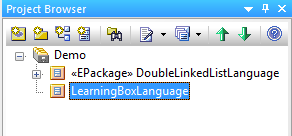
\includegraphics[width=0.55\textwidth]{EA_newPackageState}
	\caption{State after creating the new package.}
	\label{fig:new_package_completed}
\end{figure}
\FloatBarrier

\vspace{1cm}

\begin{enumerate}
\item[$\blacktriangleright$] Now click the button \texttt{New Diagram} (Fig.~\ref{fig:diagram}).
\vspace{0.5cm}

\begin{figure}[htbp]
	\centering
  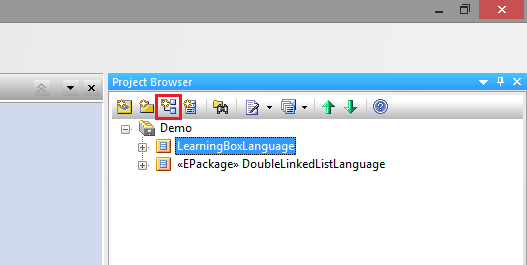
\includegraphics[width=0.72\textwidth]{EA_addDiagram}
	\caption{Add a diagram.}
	\label{fig:diagram}
\end{figure}
\FloatBarrier

\vspace{1cm}

\item[$\blacktriangleright$] In the dialog that pops up (Fig.~\ref{fig:diagram_type}), choose \texttt{eMoflon Ecore Diagrams} and \texttt{OK}.
\end{enumerate}

\vspace{1cm}

In analogy to the ``everything is an object'' principle in the OO paradigm, in metamodelling, everything is a model. \marginpar{\emph{Unification}}
This principle is called \emph{Unification} and has a lot of advantages. If everything is a model, a metamodel that defines (at least a part of) a language must be a model itself.
\marginpar{\emph{Meta-metamodel}}
\marginpar{\emph{Meta-Language}}
\marginpar{\emph{Modelling Language}}
This means that it conforms to some \emph{meta-metamodel} which defines a \emph{(meta)modelling language} or \emph{meta-language}.
For metamodelling with eMoflon, we support \emph{Ecore} as a modelling language and it defines types like \texttt{EClass} and \texttt{EReference}, which we will be using to specify  our metamodels.
Other modelling languages include MOF, UML and Kermeta.

\begin{figure}[htbp]
	\centering
  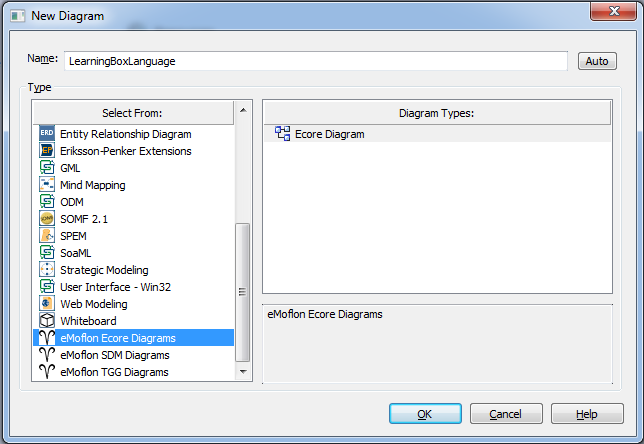
\includegraphics[width=0.8\textwidth]{EA_chooseDiagramType}
	\caption{Choose type of diagram.}
	\label{fig:diagram_type}
\end{figure}
\FloatBarrier

After creating the new diagram, your  \texttt{Project Browser} should now resemble Fig.~\ref{fig:diagram_completed}.

\begin{enumerate}
\item[$\blacktriangleright$] Double-click the newly created diagram to ensure that it is open.

\begin{figure}[htbp]
	\centering
  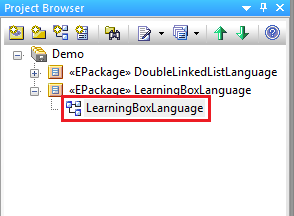
\includegraphics[width=0.5\textwidth]{EA_stateAfterDiagram}
	\caption{State after creating diagram.}
	\label{fig:diagram_completed}
\end{figure}

\item[$\blacktriangleright$] To the left of the workbench in EA, a \emph{Toolbox} should have appeared\footnote{If not, choose ``Diagram/Diagram Toolbox'' to show the current toolbox.} containing the types available in Ecore for metamodelling (Fig.~\ref{fig:eclass}).
Click on \texttt{EClass} and click in the open diagram (the main window in EA).

\begin{figure}[htbp]
	\centering
  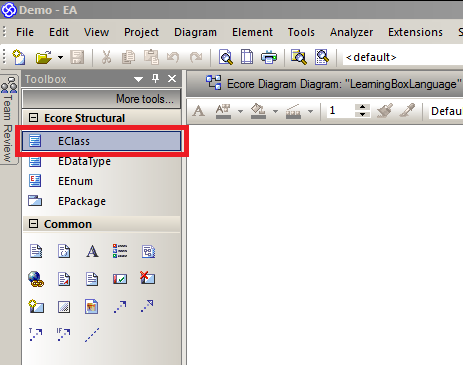
\includegraphics[width=0.7\textwidth]{EA_createEClass}
	\caption{Create an EClass.}
	\label{fig:eclass}
\end{figure}

\begin{figure}[htbp]
	\centering
  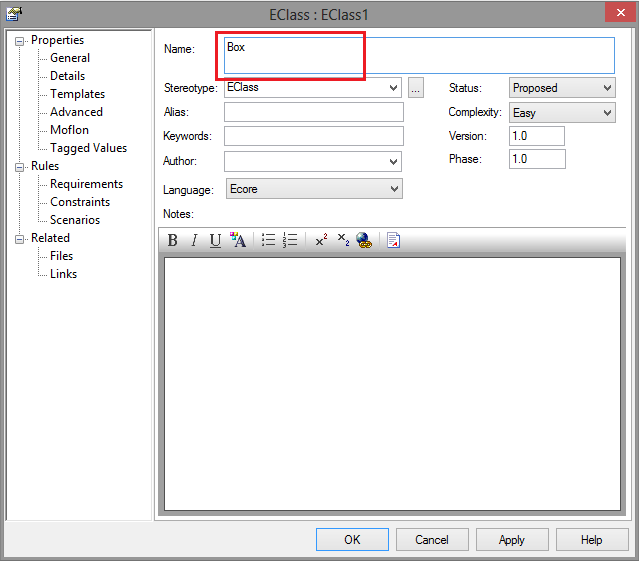
\includegraphics[width=0.6\textwidth]{EA_propertiesEClass}
	\caption{Enter properties of EClass.}
	\label{fig:eclass_properties}
\end{figure}

\item[$\blacktriangleright$] In the dialogue that pops-up, enter \texttt{Box} as the name of the class and click \texttt{OK} (Fig.~\ref{fig:eclass_properties}).
This dialogue can always be invoked by double-clicking the class and contains many other properties we'll be looking into later in the tutorial.
In general, a similar ``properties'' dialogue can be opened in the same fashion for almost every element in EA.

\item[$\blacktriangleright$] After creating \texttt{Box}, your EA workspace should resemble Fig.~\ref{fig:eclass_completed}.

\begin{figure}[htbp]
	\centering
  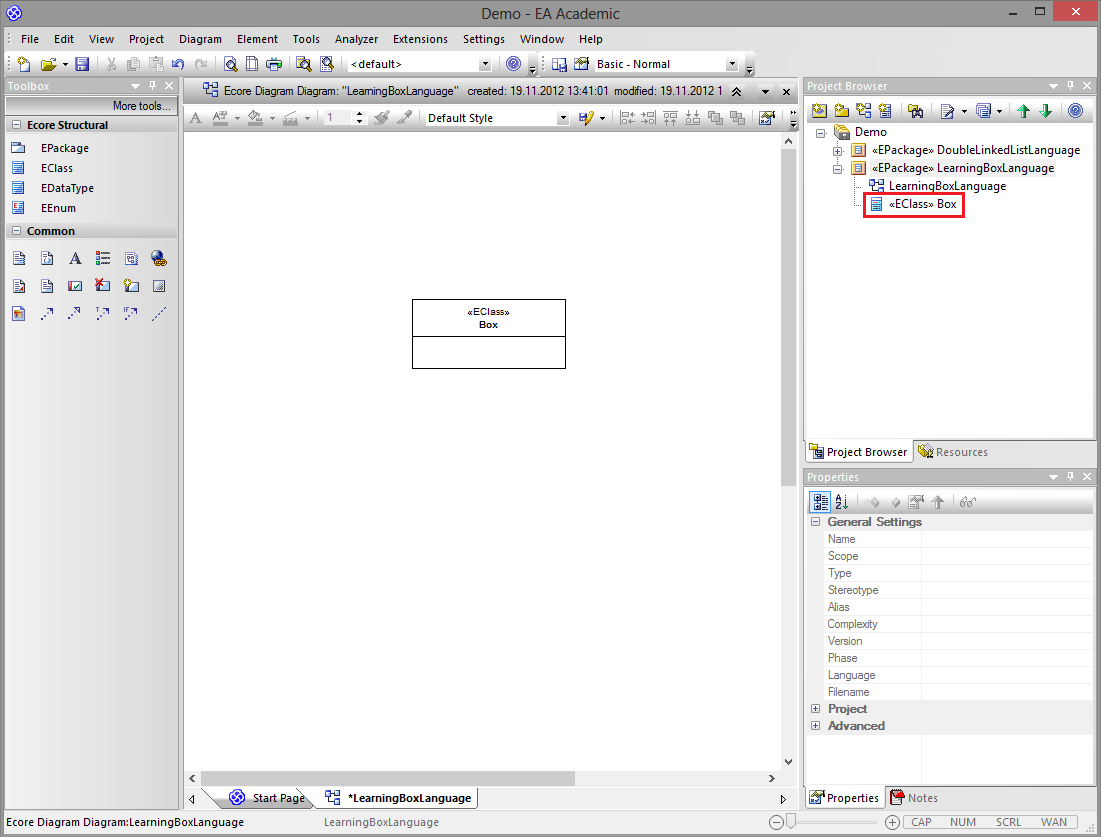
\includegraphics[width=0.7\textwidth]{statePostCreation}
	\caption{State after creating \texttt{Box}.}
	\label{fig:eclass_completed}
\end{figure}


\item[$\blacktriangleright$] Now create \texttt{Partition} and \texttt{Card} in the same way, until your workspace resembles Fig.~\ref{fig:all_eclasses}.
These are the main classes for our learning box.

\begin{figure}[htbp]
	\centering
  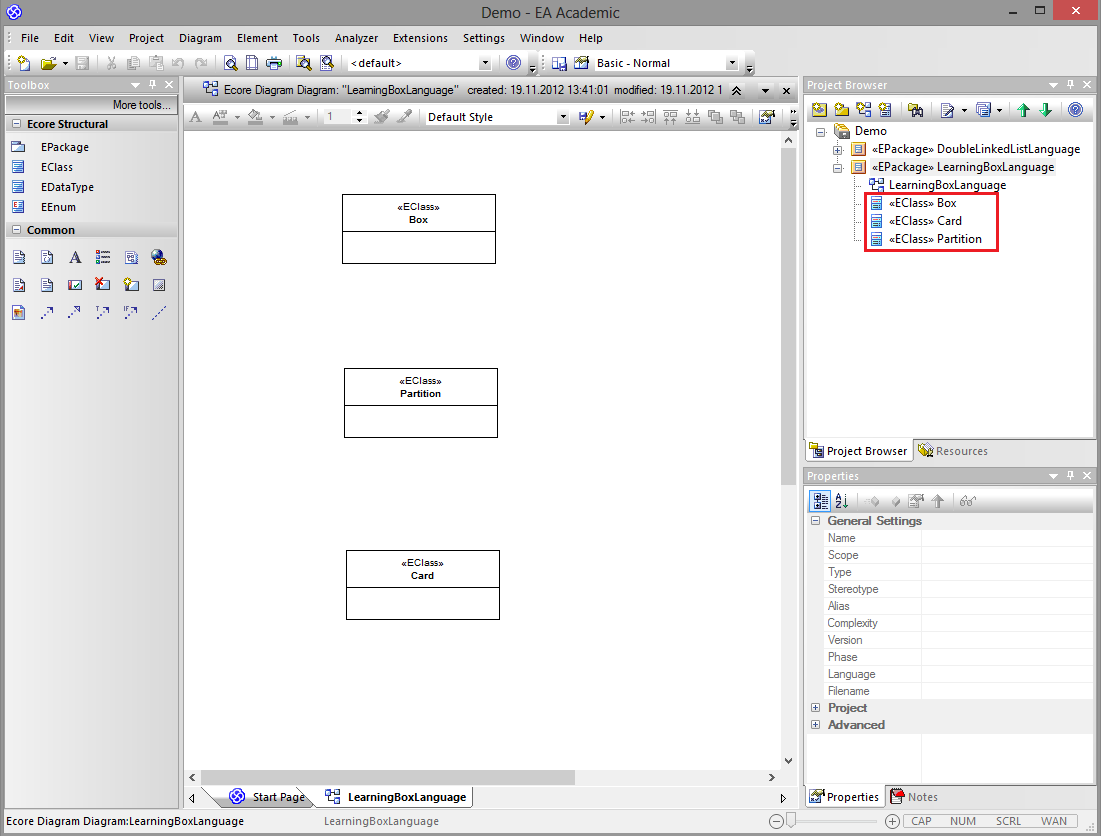
\includegraphics[width=0.7\textwidth]{EA_createPartitionCard}
	\caption{Main classes in our metamodel.}
	\label{fig:all_eclasses}
\end{figure}

\pagebreak

\item[$\blacktriangleright$] Now choose \texttt{Box}, right-click to call up the context menu and choose ``Features \& Properties/Attributes..'' (Fig.~\ref{fig:attribute}).

\begin{figure}[htbp]
	\centering
  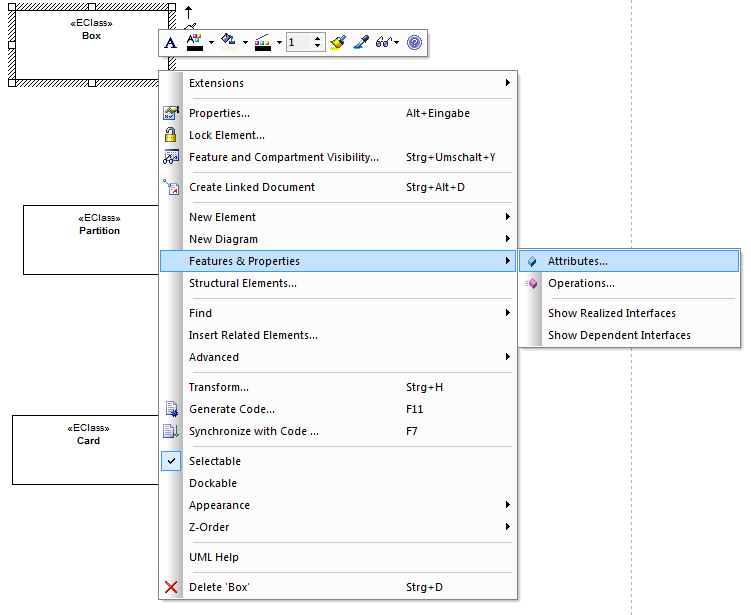
\includegraphics[width=0.6\textwidth]{EA_contextAddAttribute}
	\caption{Context Menu for a class.}
	\label{fig:attribute}
\end{figure}
\FloatBarrier

\vspace{0.5cm}

\item[$\blacktriangleright$] In the dialogue that pops-up, enter \texttt{name} as the name of the attribute, choose \texttt{EString} as its type and press \texttt{Save} (Fig.~\ref{fig:attribute_properties}).
A new attribute for the same class can be added by choosing \texttt{New}.

\vspace{0.5cm}

\begin{figure}[htbp]
	\centering
  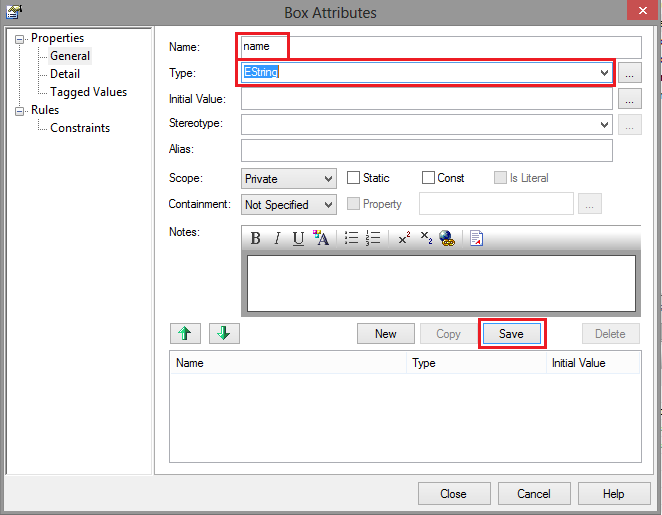
\includegraphics[width=0.75\textwidth]{EA_addingAttributes}
	\caption{Adding attributes to a class.}
	\label{fig:attribute_properties}
\end{figure}

\pagebreak

\item[$\blacktriangleright$] Add attributes to the other classes until your workspace resembles
Fig.~\ref{fig:attribute_completed}.

\begin{figure}[htbp]
	\centering
  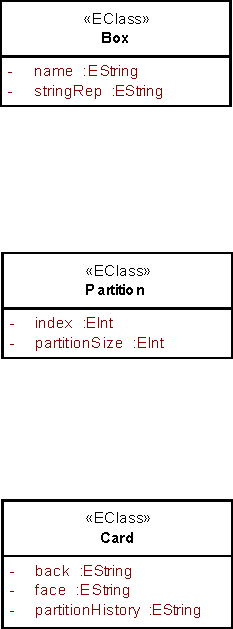
\includegraphics[width=0.25\textwidth]{EA_allAttributes}
	\caption{Main classes with attributes.}
	\label{fig:attribute_completed}
\end{figure}
\FloatBarrier

\item[$\blacktriangleright$] A fundamental gesture in EA is \emph{Quick Link}.
Quick Link is used to create links between elements in a context sensitive manner.
To use Quick Link, choose an element and note the little black arrow in its top-right corner (Fig.~\ref{fig:quicklink}).

\begin{figure}[htbp]
	\centering
  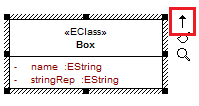
\includegraphics[width=0.4\textwidth]{EA_quickLink}
	\caption{Quick Link is a central gesture in EA.}
	\label{fig:quicklink}
\end{figure}
\FloatBarrier

Now click on the black arrow and pull to another element you wish to ``quick link" to.
In this case quick link from \texttt{Box} to \texttt{Partition}.
In the context-menu that pops-up, choose \texttt{Create Bidirectional EReference} (Fig.~\ref{fig:ereference}).

\begin{figure}[htbp]
	\centering
  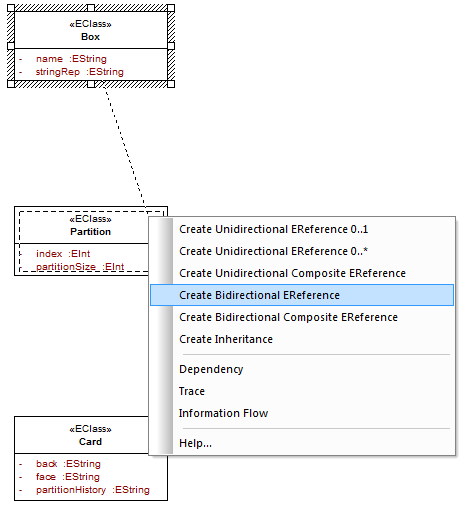
\includegraphics[width=0.5\textwidth]{EA_ereferenceBidirectional}
	\caption{Create a reference via Quick Link.}
	\label{fig:ereference}
\end{figure}
\FloatBarrier

\item[$\blacktriangleright$] Double click the reference to invoke a dialogue. %(Fig.~\ref{fig:ereference_properties}). 
Here you can change the reference direction\footnote{this is particuluary useful if you accidentally click one of the other options while creating the quick link and wish to change it.} and enter a name. The name will only be used for documentation purpose as it is not relvant for code generation.

% \begin{figure}[htbp]
% 	\centering
%   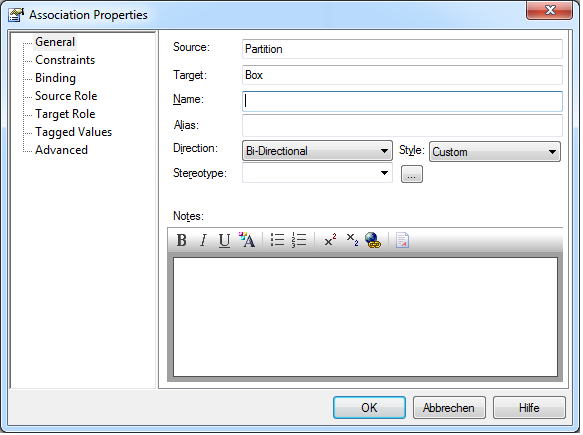
\includegraphics[width=0.6\textwidth]{EA_propertiesBidirectional}
% 	\caption{Enter properties of the reference.}
% 	\label{fig:ereference_properties}
% \end{figure}

% Do BOX (target) first..
\item[$\blacktriangleright$] In the same dialogue choose \texttt{Target Role} and enter the values in Fig.~\ref{fig:reference_ends} to set the properties for the ``target'' end of the reference (the \texttt{Box} role). As you can see, the default target is set to the class you linked \emph{from}, and the default source is the class you linked \emph{to}. If you decided to ignore the instructions, and went from \texttt{Partition} to \texttt{Box}, the only difference between the references are the titles - The following information will still be the same! In this window, it's important not to forget to check and modify the \texttt{Role}, \texttt{Multiplicity}, \texttt{Aggregation} and \texttt{Navigability} settings for the source.  Repeat the process for the \texttt{Source Role}.

\begin{figure}[htbp]
	\centering
	  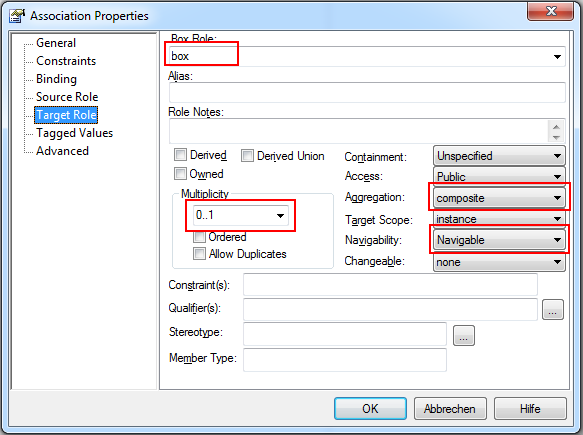
\includegraphics[width=0.8\textwidth]{EA_assocPropsTarget}\\
  \vspace{0.5cm}
    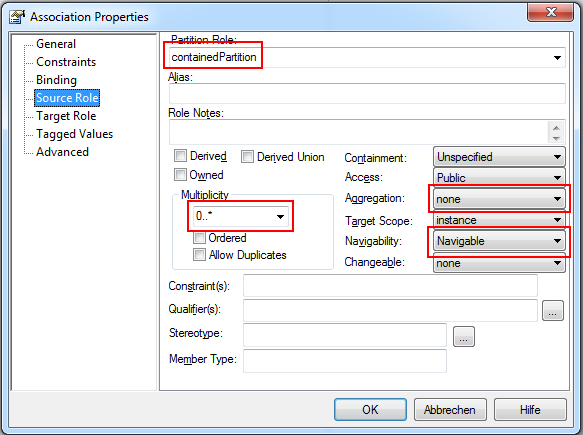
\includegraphics[width=0.8\textwidth]{EA_assocPropsSource}
	\caption{Enter properties for target and source of reference.}
	\label{fig:reference_ends}
\end{figure}
\FloatBarrier
\end{enumerate}

Navigable ends are mapped to class attributes with getters and setters in Java and therefore \emph{must} have a specified name and  multiplicity for successful code generation.
Corresponding values for non-navigable ends can  be regarded as additional documentation and do not have to be specified.

The multiplicity of a reference controls if the relation is mapped to a Java Collection (\texttt{*},  \texttt{1..*}, \texttt{0..*}), or a single valued class attribute (\texttt{1}, \texttt{0..1}).

In Ecore, the aggregation values of a reference can either be \texttt{none} or \texttt{com\-po\-site}.
Composite means that the current role is that of a \emph{container} for the opposite role.
In our case for example, \texttt{box} is a container for \texttt{partitions}.\\
This has a series of consequences: (1) every element must have a container, (2) an element cannot be in more than one container at the same time, and (3) a container's contents are deleted together with the container.
Non-composite (\texttt{none}) means that the current role is not that of a container and the rules for containment do not hold (reference is a simple ``pointer'').

If you've done everything right, your workspace should now resemble Fig.~\ref{fig:ereference_completed} with a relation between \texttt{Box} and \texttt{Partition}.

\begin{figure}[htbp]
	\centering
  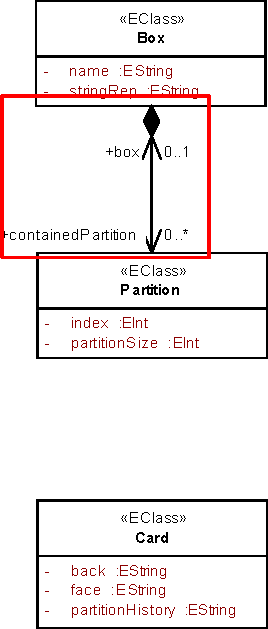
\includegraphics[width=0.33\textwidth]{EA_relationBoxPartition}
	\caption{\texttt{Box} contains \texttt{Partition}s.}
	\label{fig:ereference_completed}
\end{figure}
\FloatBarrier

\begin{enumerate}
\item[$\blacktriangleright$] Create a bidirectional reference\footnote{To be precise, \emph{all} references in Ecore are actually unidirectional.
A ``bidirectional'' reference in our metamodel is in reality mapped to two \texttt{EReferences} that are opposites of each other.
We however believe it is simpler to handle these pairs as single references and prefer this concise concrete syntax.} between \texttt{Partition} and \texttt{Card} and two unidirectional self-references for \texttt{Partition} according to Fig.~\ref{fig:ereferences_all}\footnote{If you have difficulties deciphering the role names and other details in the screen shot please refer to Fig.~\ref{fig:metamodel_complete} for a better diagram of the metamodel.}.

\begin{figure}[htbp]
	\centering
  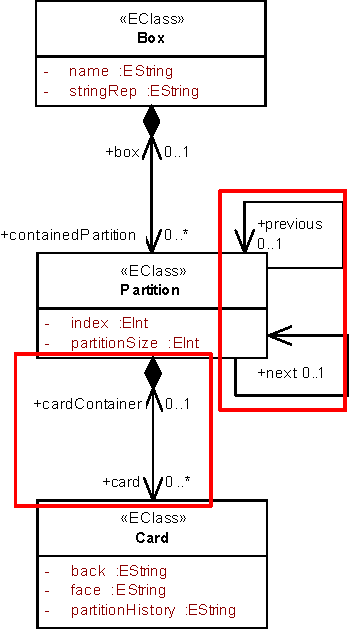
\includegraphics[width=0.5\textwidth]{EA_relationsAll}
	\caption{All relations in our metamodel.}
	\label{fig:ereferences_all}
\end{figure}
\end{enumerate}
\FloatBarrier

All of your program attributes and references have now been set up. To see how this would appear in eMoflon's textual syntax, check out figure~\ref{fig:allReferences} and \ref{fig:partitionReferences} from section~\ref{sec:staticConcrete} 

Every system has, in addition to its static structure, certain dynamic aspects that describe the system's behaviour and how it evolves over time or reacts to external stimulus.
\marginpar{\emph{Dynamic Semantics}}
In a language, these rules that govern the dynamic behaviour of a system are referred to collectively as the \emph{Dynamic Semantics} of the language.
Although these rules can be defined as a set of separate \emph{Model Transformations}, we take a holistic approach and advocate integrating the transformations directly in the metamodel as operations.
This fits nicely to the object-oriented paradigm and is quite natural in many cases.

In the next few steps we shall define the \emph{signatures} of some operations for our learning box.
We will use SDMs in a later handbook to \emph{implement} these methods.
\begin{enumerate}
\item[$\blacktriangleright$] Right-click \texttt{Partition} to invoke the context-menu depicted in Fig.~\ref{fig:add_operation} and choose ``Features \& Properties/Operations..''.

\begin{figure}[htbp]
	\centering
  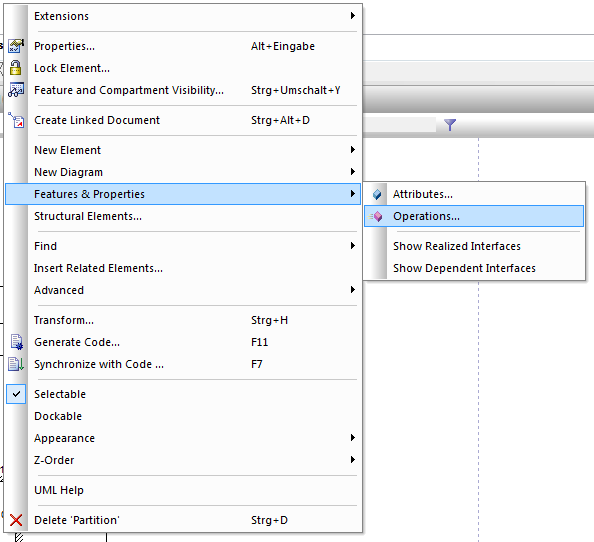
\includegraphics[width=0.55\textwidth]{EA_contextAddOperation}
	\caption{Add an operation.}
	\label{fig:add_operation}
\end{figure}
\FloatBarrier

\item[$\blacktriangleright$] In the dialogue that pops-up (Fig.~\ref{fig:operation_properties}), enter \texttt{empty} as the \texttt{Name} of the operation, leave the \texttt{Return Type} as \texttt{void}.  Press \texttt{Save}.

\begin{figure}[htbp]
	\centering
  	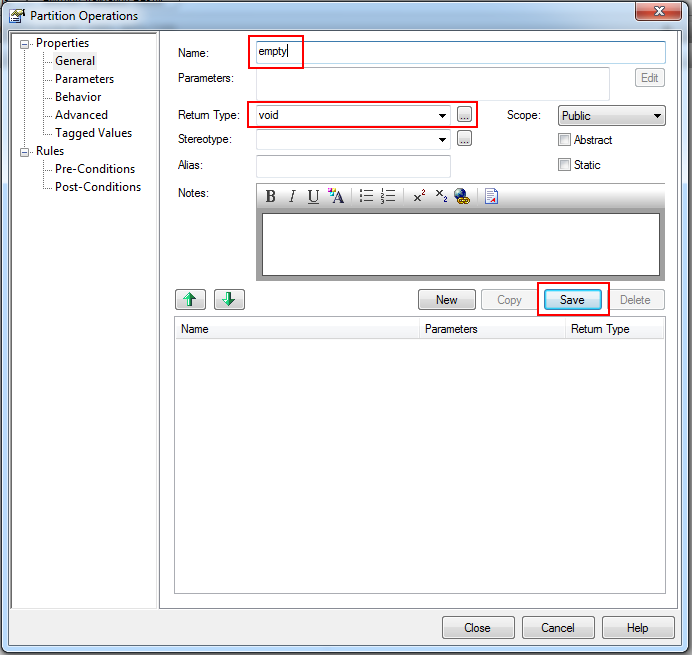
\includegraphics[width=0.6\textwidth]{EA_operationEmpty}
	\caption{Properties for operation.}
	\label{fig:operation_properties}
\end{figure}
\FloatBarrier

\item[$\blacktriangleright$] In the same dialogue, press \texttt{New} to add further operations and enter the values in Fig.~\ref{fig:operation_parameters}.  Parameters can be added by pressing \texttt{Edit}\footnote{You must save the operation before this option will become active.} and entering the name and choosing the type of each parameter in a separate dialogue. Don't forget to save everything!

\begin{figure}[htbp]
	\centering
  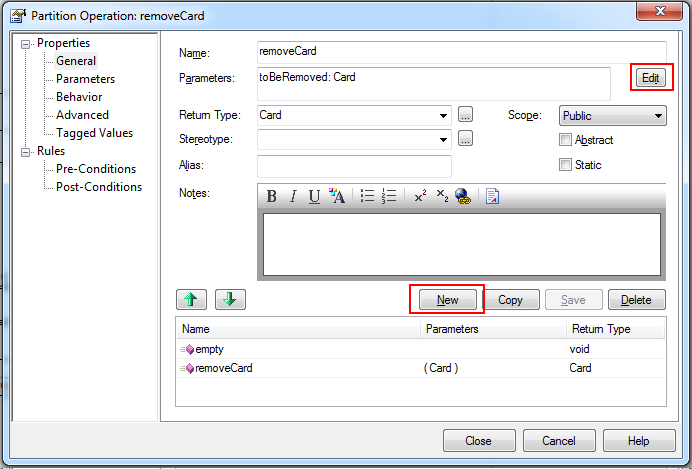
\includegraphics[width=0.85\textwidth]{EA_operationRemoveCard}
	\caption{Parameters and Return Type.}
	\label{fig:operation_parameters}
\end{figure}
\FloatBarrier

\item[$\blacktriangleright$] Repeat the process for the \texttt{check} operation in Fig.~\ref{fig:operation_partition}.
Notice that the \texttt{Return Type} can be chosen via the drop-down menu for primitives (e.g. \texttt{EBoolean}), or via the `\texttt{\ldots}' button (indicated in Fig.~\ref{fig:operation_parameters}) for types you've established in the metamodel (e.g. \texttt{Card}).
\end{enumerate}

\vspace{-.5cm}
\begin{quote}
$\textbf{Please note:}$ Non-primitive types \emph{must} be chosen via the `\texttt{\ldots}' button. It allows you to browse for the corresponding elements in your project. Unfortunately, just typing them won't work!
\end{quote}
\vspace{-.5cm}

\pagebreak

\begin{figure}[htbp]
	\centering
  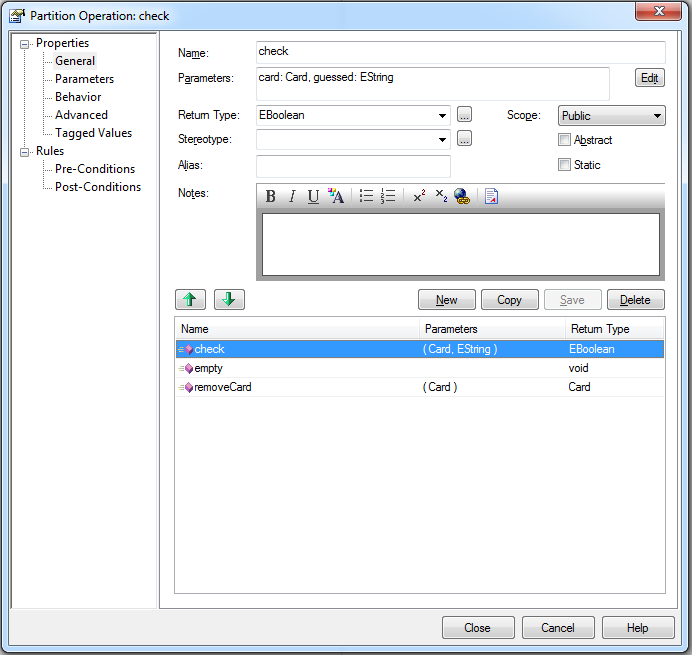
\includegraphics[width=0.9\textwidth]{EA_operationCheck}
	\caption{All operations in \texttt{Partition}.}
	\label{fig:operation_partition}
\end{figure}

If you've done everything right, your dialogue should now contain three methods: \texttt{check}, \texttt{empty}, and \texttt{removeCard}, each with corresponding parameters and return types as in Fig.~\ref{fig:operation_partition}.

Add all operations analogously for \texttt{Box} and \texttt{Card}, so that your metamodel closely resembles Fig.~\ref{fig:metamodel_complete}.

\begin{figure}[htbp]
	\centering
  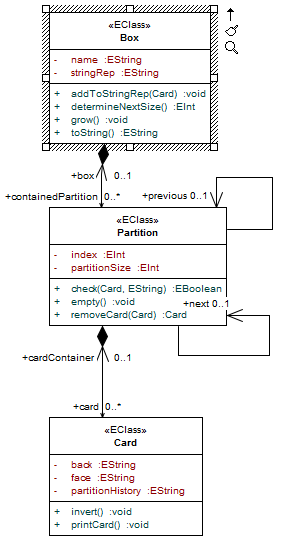
\includegraphics[width=0.7\textwidth]{EA_metamodelComplete.png}
	\caption[Complete metamodel for our learning box.]{Complete metamodel for our learning box (please note that names of method parameters may not be displayed by default in EA, but are shown here for presentation purposes).}
	\label{fig:metamodel_complete}
\end{figure}


Lets take a step back and review our metamodel.
We have modelled a \texttt{Box} that contains arbitrary many \texttt{Partition}s.
A \texttt{Partition} in the \texttt{Box} has a \texttt{next} and \texttt{previous} \texttt{Partition} that can be set or not. Finally, \texttt{Partition}s contain \texttt{Card}s.

A \texttt{Box} has a \texttt{name}, and can be extended by calling \texttt{grow}.
A \texttt{Box} can print out its contents via \texttt{toString}.

The main method of the learning box is \texttt{Partition::check} that takes a \texttt{Card} and the user's guess as an \texttt{EString} and returns \texttt{true} or \texttt{false} depending on if the guess was correct or not.

\pagebreak 

A \texttt{Partition} can also \texttt{empty} itself of all \texttt{Cards}, or \texttt{remove} a particular \texttt{Card}.
Last but not least, a \texttt{Partition} has a \texttt{partitionSize} that can be used to indicate that the \texttt{Partition} is full and is ready to be revised.

A \texttt{Card} contains the actual content to be learnt as a question on the card's \texttt{face} and the answer on the card's \texttt{back}.
A \texttt{Card} also maintains a \texttt{partition\-History} which can be used to keep track of how often a \texttt{Card} has been answered correctly/wrongly.
This might indicate how difficult the \texttt{Card} is for a specific user.
When learning a language, it makes sense to be able to swap the target and source language and this is supported by \texttt{Card} via \texttt{invert} (turns the card around).

To see how this complete metamodel is depicted using the textual syntax, check out figure~\ref{fig:workspaceMethods} from section~\ref{sec:staticConcrete}

Now try to export the metamodel for code generation in Eclipse (if problems occur during the following steps, we recommend reading \texttt{Part VI: Micellaneous}. This might help you to find your mistakes).

\begin{enumerate}
\item[$\blacktriangleright$] To do this, right-click on \texttt{LearningBoxLanguage} and choose ``Extensions/MOFLON::Ecore Addin/Export Selection to Workspace''.
Then switch to your Eclipse work\-space and refresh the metamodel workingset. Alternatively, you can activate eMoflon's add-in window by going to ``Extensions/Add-in Windows,'' and pressing \texttt{All} in the \texttt{Export} box.
\end{enumerate}


If you have done everything right, a new project \texttt{LearningBoxLanguage} should be created in the \texttt{Demo} working set within your Eclipse workspace.
If this is not the case, please ensure that your metamodel is identical with Fig.~\ref{fig:metamodel_complete}.

If you believe everything is correct and things still don't work, then feel free to contact us at \href{mailto:contact@moflon.org}{contact@moflon.org}.

If code is generated successfully, take a look at all the stuff that's been generated under \texttt{/gen}. Especially look at the the default implementation for all methods who throw an  \texttt{OperationNotSupported} exception.
We shall see later in the handbook that the EMF code generator actually supports injecting hand-written implementations of methods into generated methods and classes.
With eMoflon however, we can also model a large part of the dynamic semantics, and only need to implement small helper methods (e.g. string manipulation) by hand.

\fancyfoot[R]{ $\triangleright$ \hyperlink{validation vis}{Next task} }